\chapter{Девять жизней Асафа Бен-Нуна}

В качестве основы статьи взято интервью главного героя одному израильскому блогу (ссылка ниже). Комментарии, перевод - мои.

Было уже темно, когда половина Галилеи (область на севере Израиля — А.Н.) затаила дыхание. Горящий израильский самолёт возвращается из Сирии, снижаясь, и пытается дотянуть до Аелет Хашахар (киббуц в 5 км. от границы с Сирией - А.Н), а затем резко пикирует и с грохотом врезается в поле, над которым появляется огромный гриб. Несколько секунд беспокойства, и огромное облегчение — в небе появляется белый парашют. В этом сюжете появляется новый поворот — сильный западный ветер тянет его назад, в Сирию. Откуда по лётчику начинают стрелять, кажется, из всего, что есть под рукой. Сможет ли он благополучно приземлиться в Израиле, или будет убит — в небе, или сирийском плену?

Сейчас этот пилот находится в Неве-Цедек, в Тель-Авиве. 80-летний Асаф Бен-Нун, ветеран ВВС с впечатляющим послужным списком: пять войн, в которых он собрал 2700 часов налёта на истребителях. Начиная с «Мустанга», Урагана, Метеора и Норда, продолжая «Гарвардом», «Мистером», «Фугой» и F-15. Надеюсь, он простит нам, что мы забыли 15 других самолётов, на которых он летал. На его счету пять сбитых самолётов МиГ — МиГ-17 в Шестидневную и четыре МиГ-21 в войну Йом-Киппур. И дважды он был сбит сам.

Асаф — младший брат Йохая Бен-Нуна, героя Израиля 1948 года, основателя Шайетет-13 («13-я флотилия», флотский спецназ - А.Н.), и главкома ВМФ в 60-х годах. Асаф радился в Бейт-Хакереме в Иерусалиме, а затем переехал в киббуц Бейт-Хашита. «Мой брат был удивительным человеком, которого я любил и которым восхищался» — говорит Асаф, который на десять лет младше своего брата. Он говорит, что Йохай хотел, чтобы его брат стал боевым пловцом. Тогда они тренировались под руководством итальянев Фиоронзо Каприотти, ветеранов 10-й флотилии МАС (знаменитые боевые пловцы князя Боргезе — А.Н.). Во Вторую Мировую они потопили несколько английских кораблей. «Раньше я ездил с братом на практику в Сдот-Ям и занимался там дайвингом. Мне сложно было поверить — как эти парни могу так много времени проводить под водой!»

Почему ты не пошел во флот?- «В 1953 году, когда меня призвали, меня не взяли на курс морских офицеров из-за шумов в моём сердце. Но через год проблема была решена, и я попал на лётный курс. Я летал до 60 лет»

Во время Синайской компании (1956 год) он был молодым лётчиком эскадрилии «Мустангов» из Рамат-Давида. Первый же боевой вылет едва не стал для него последним. «Мустанги» атаковали колонну египетской бронетехники в Абу-Агейле, и в одной из атак в топливный бак его самолёта попала пуля. Бен-Нун вспоминает: «Остекление кабины было забрызгано маслом, и я понял, что самолёт вот-вот станет неуправляемым. Я пересек границу, и в этот момент двигатель заглох. Я присмотрел поле для посадки, самолёту понадобилось всего десять метров, чтобы остановиться. Крылья были серьёзно повреждены, как и винт, но я почти не пострадал. Наши солдаты быстро нашли меня».

\begin{figure}[h!tb] 
	\centering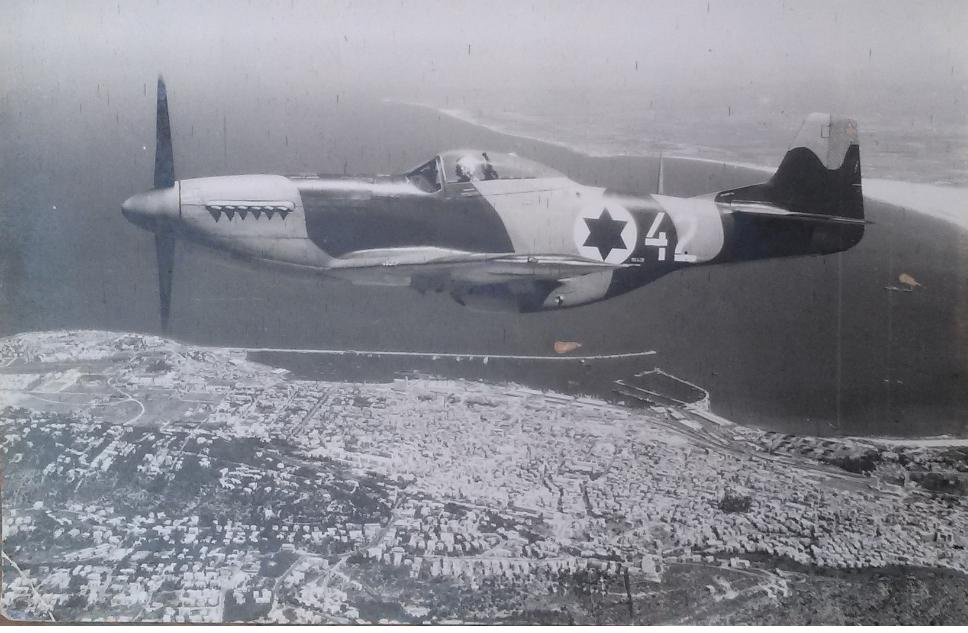
\includegraphics[scale=0.5]{History_BenNun/eWF3hz6vz80.jpg}
	%	\label{fig:scipion} % Unique label used for referencing the figure in-text\end{document}
	%	%\addcontentsline{toc}{figure}{Figure \ref{fig:placeholder}} % Uncomment to add the figure to the table of contents%----------------------------------------------------------------------------------------
	\caption{1956, Ассаф Бен-Нун в Мустанге над заливом Хайфы. В Синайской кампании его самолет был поражен, и он совершил вынужденную посадку в районе Рафаха}%	CHAPTER 2
\end{figure}

Во время Синайской компании было много разного, но наш рассказ о Шестидневной войне. В 1957 году он переучился на Мистер (Dassault Mystère IV, франуцзский истребитель-бомбардировщик 50-х годов — А.Н). Во время обучения я провёл шесть месяцев во Франции. В конце 1950-х годов Асаф был лидером пилотажной группы, летавшей на Гарвардах. В 1960-м году он уволился из ВВС в запас, вернулся в Бейт-Хашиту и продолжал летать как резервист: «Это было настоящее открытие, актуальное и по сегодняшний день - боевые лётчики-резервисты не хуже тех, кто на действительной службе. Это означает, что ты летаешь один раз в неделю и поддерживаешь свои навыки».

В то же время Бен-Нун стал лётчиком-испытателем в IAI. Это быо его основной профессией, когда он начал изучать авиационную технику в Технионе в 1964 году. Во время учебы случилась Шестидневная война. В то время ему было 32 года, он женился и жил в Хайфе.

\begin{figure}[h!tb] 
	\centering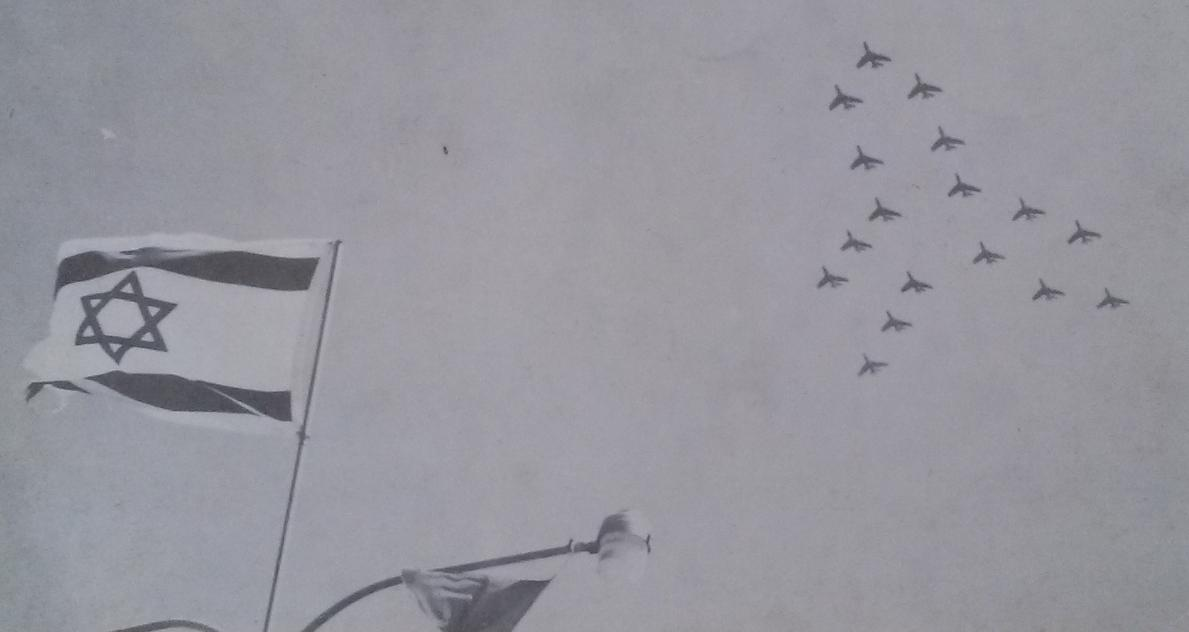
\includegraphics[scale=0.4]{History_BenNun/SFrAwIWTjoA.jpg}
	%	\label{fig:scipion} % Unique label used for referencing the figure in-text\end{document}
	%	%\addcontentsline{toc}{figure}{Figure \ref{fig:placeholder}} % Uncomment to add the figure to the table of contents%----------------------------------------------------------------------------------------
	\caption{1959, Бен-Нун на авиашоу}%	CHAPTER 2
\end{figure}

Бен-Нун: «Я был в 109-й эскадрилье «Мистеров» в Рамат-Давиде, её командиром был Охад Шадми, мой ровесник, когда нам поступили задачи первого дня войны. Мы долго тренировались атаковать цели на Синае, планировали атаку и распределяли цели на египетских аэродромах между собой. 5 июня я был в первой волне, атаковавшей египетские аэродромы, и у каждого из нас было 5-6 минут над целью для атаки, после чего мы уступали место следующей волне»

\begin{figure}[h!tb] 
	\centering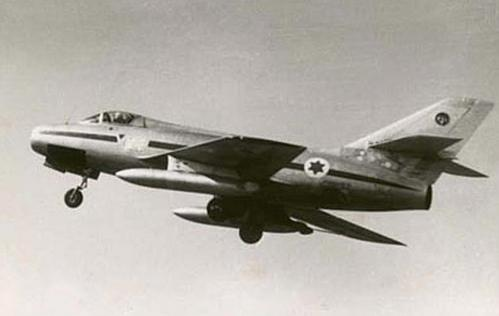
\includegraphics[scale=0.8]{History_BenNun/VsBbAb7luwA.jpg}
	%	\label{fig:scipion} % Unique label used for referencing the figure in-text\end{document}
	%	%\addcontentsline{toc}{figure}{Figure \ref{fig:placeholder}} % Uncomment to add the figure to the table of contents%----------------------------------------------------------------------------------------
	\caption{«Мистер» на котором Бен-Нун сбил МиГ-17}%	CHAPTER 2
\end{figure}

«Мы подходили к цели со стороны моря на очень маленькой высоте, пересекли озеро Бардавиль, там ещё были египетские рыбацкие лодки, а потом пять минут атаковали взлётно-посадочные полосы и их самолёты, которые стояли рядами у основания полос. Нам приказали возвращаться, и в тот момент меня атаковал египетский МиГ-17. Проблема в том, что это гораздо более манёвренный самолёт, у него есть форсаж, и просто — он в несколько раз лучше, чем «Мистер». Но мне удалось его сбить, хоть я и остался практически без топлива и чудом сумел дотянуть до Тель-Ноф (авиабаза существенно ближе к границе с Египтом, чем «родной» для 109-й Рамат-Давид).

В тот день Бен-Нун совершил ещё два вылета — в Бир Тамаду и Файяд. На следующий день, во вторник, 6 июня, он вылетал ещё трижды — в Бир Лахафан, в Иерусалим и Аль-Азарию, а также в район Бир-Гафгафа (крупная египетская авиабаза, в дальнейшем — Рефидим — А.Н.). 7 июня он начал с атаки на иракскую бронетехнику в районе Иерусалим-Иерихон. Вторая миссия была в Сирии, а третий вылет стал для него судьбоносным.

Это произошло во второй половине дня 7 июня 1967 года. Накануне, после тяжелого артобстрела, сирийцы попытались захватить кибуц Дан и район Ашмуры. Попытка была сорвана. Целью Бен-Нуна было атаковать танки в районе Старой Таможни. Четвёрка «Мистеров» вылетела из Рамата Давида во главе с самолётом №14 капитана Бен-Нуна, возглавлявшего группу.

Он рассказывает: «На западе от здания Таможни было поле, где я увидел группу танков, которые атаковал напалмом и 250-килограммовыми бомбами. Каждый самолет имеет пару баков, вы бросаете их с очень низкой высоты, буквально 50 метров. Она горит, как коктейль Молотова. Мы прошлись по ним напалмом, и мои номера 3 и 4 немного отдалились от меня. Мы летели двумя парами, и они не смогли найти цель, потому что сирийские танки были вкопаны. Один танк, на который я атаковал, уже горел, но они не видели других. Поэтому я сказал им: «Хорошо, сделаем ещё один заход. И в этой атаке меня подбили». 

\textit{Это был взрыв?}

«Что-то ударило меня с земли, я не знаю, что. Сразу же двигатель заглох, и вспыхнул пожар. Я не видел огня, но есть лампочка, предупреждающая вас, что вы горите, и ребята позади тоже видели пламя. Но я действительно не хотел прыгать над Сирией. У меня было достаточно скорости, я тянул к западу, пересекая границу, они кричали мне, чтобы я катапультировался, и я знаю, что там обычно сильный западный ветер. Я покинул самолёт примерно над киббуцем Аелет Хашахар, когда самолёт стал неуправляемым, и в этот момент я прыгнул».

\begin{figure}[h!tb] 
	\centering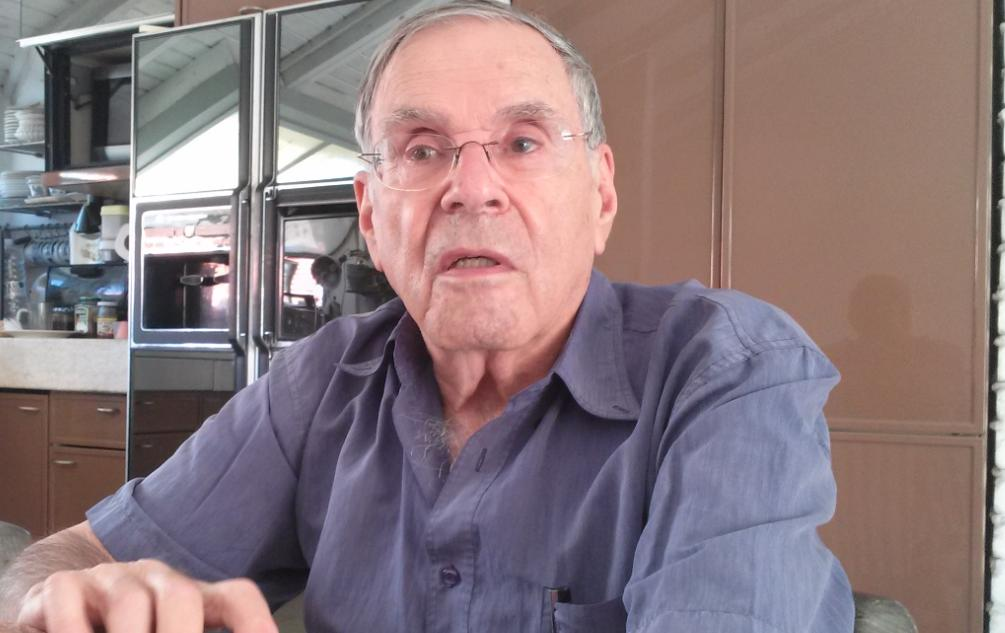
\includegraphics[scale=0.4]{History_BenNun/k2t_Wfyj1Lw.jpg}
	%	\label{fig:scipion} % Unique label used for referencing the figure in-text\end{document}
	%	%\addcontentsline{toc}{figure}{Figure \ref{fig:placeholder}} % Uncomment to add the figure to the table of contents%----------------------------------------------------------------------------------------
	\caption{Тель-Авив. Ассаф Бен-Нун у себя дома в Неве Цедек. }%	CHAPTER 2
\end{figure}

\textit{Как ты катапультировался?}

«Я был довольно высоко, на 3000 футах (900 метров — А.Н.), и тут - ваше кресло вылетает. В наше время для этого есть реактивные ускорители, но тогда это было похоже на пушку, и удар был ужасен. Все мы проходили парашютный курс в лётной школе, но он не готовил к такому. Это было моё первое катапультирование.

\textit{Не очень приятно.}

Я почувствовал сильный удар. Если вы ниже 14000 футов, то ваше кресло будет отброшено, и парашют автоматически откроется. Так что я обнаружил себя висящим на парашюте и дрейфующим в сторону Сирии. На этой высоте вы не чувствуете, как приближается земля. Я был уверен, что спущусь на землю уже в Сирии.

\textit{И они стреляли в тебя?}

Я слышал свист пуль вокруг. 

\begin{figure}[h!tb] 
	\centering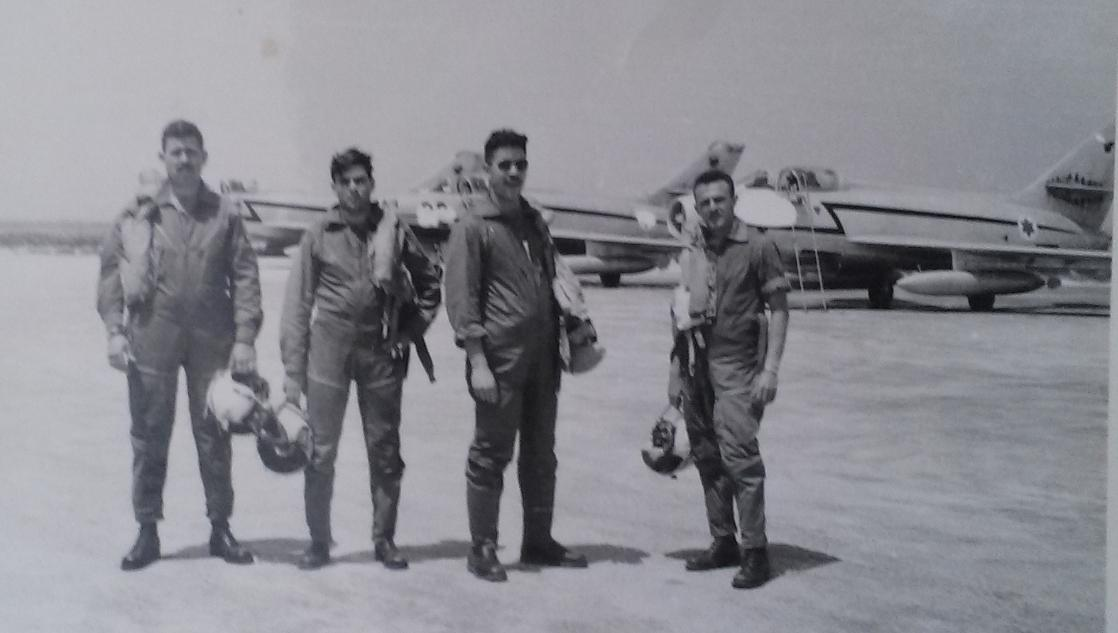
\includegraphics[scale=0.4]{History_BenNun/Sch3Sv1MZmY.jpg}
	%	\label{fig:scipion} % Unique label used for referencing the figure in-text\end{document}
	%	%\addcontentsline{toc}{figure}{Figure \ref{fig:placeholder}} % Uncomment to add the figure to the table of contents%----------------------------------------------------------------------------------------
	\caption{Ассаф Бен-Нун [второй слева] в эскадрилье 109 в Рамат-Давиде }%	CHAPTER 2
\end{figure}

\textit{Вы смотрели, откуда по вам стреляют и где вы находитесь?}

«Да, я все время смотрел».

\textit{А граница - река Иордан.}

«Я видел реку, и точно знал, где я нахожусь. В своё время я облетел всю Верхнюю Галилею и знал эту область, как свои пять пальцев».

\textit{Вы падали минуту или две?}

«Я думаю больше, может быть, три минуты, и, к счастью, я приземлился на нашей стороне. Когда-то сирийцы хотели отвести воды Иордана, и мы вырыли здесь траншеи, буквально в 10-20 метрах от реки. Мне повезло, что я угодил в них — сирийцы не могли по мне стрелять.

\textit{Какое оружие у вас было?}

«У меня был пистолет и нож, и как только я упал в канаву, я перерезал несколько строп, чтобы освободиться. Я всё ещё был очень близко к границе. Когда я побежал оттуда, они снова начали стрелять по мне снова, так что мне пришлось какое-то время сидеть в окопе. Потом я услышал голоса. Я всё ещё боялся, что это сирийцы, так что я достал пистолет и стал ждать их».

\textit{Вы считали, что это сирийцы, хотя вы приземлились на израильскую сторону?}

«Да, послушай, это война, и ты не знаешь, пересекли сирийцы границу или нет. Потом я понял, что это были наши ребята. Парни из общин на севере, киббуцники из Шамира, Лехавот Шабашан. Я был полностью измотан, когда они вытащили меня из окопа».

\textit{Под огнем?}

«Сирийцы продолжали стрелять, мы были как на ладони». 

\begin{figure}[h!tb] 
	\centering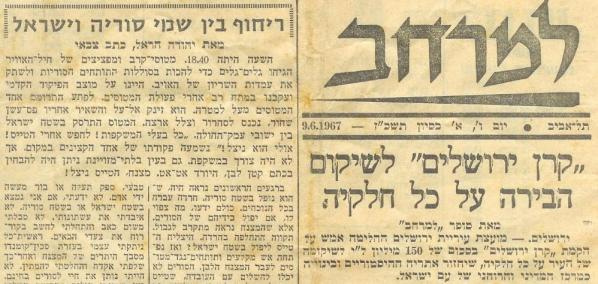
\includegraphics[scale=0.6]{History_BenNun/ODbl5G862D4.jpg}
	%	\label{fig:scipion} % Unique label used for referencing the figure in-text\end{document}
	%	%\addcontentsline{toc}{figure}{Figure \ref{fig:placeholder}} % Uncomment to add the figure to the table of contents%----------------------------------------------------------------------------------------
	\caption{«Парящий между небом и землей» в газете «Ламерхав». }%	CHAPTER 2
\end{figure}

На прошлой неделе в газете «Ламерхав» пресс-секретарь IDF Иегуда Харель сообщил, что время, когда самолет был сбит — 8:40: «Мы были на передовом командном пункте на горе Кнаан, и мы очень нервничали по поводу действий самолетов. Внезапно один из самолетов поднялся выше цели. Он оставлял полосу черного дыма. Самолет разбился на израильской территории между общинами долины Хула. «Ищите пилота! Может быть, он спасся!» — был слышен приказ одного из офицеров. Но даже невооруженным глазом можно было увидеть, как белое пятно медленно опускается. Это был парашют, пилот был спасен. В первые минуты он, казалось, падал на территории Сирии. Все боялись за него. Все знали, что с ним случится, если он попадет в руки сирийцев. Но парашют, кажется, приближается к границе. Надежда обратилась в беспокойство. Удастся ли пилоту остаться на израильской земле? Затем по белому парашюту открыли огонь из пулемётов и зенитных орудий. Сирийцы не могли смириться с тем, что израильский пилот сумел уцелеть даже после того, как его самолет упал. Мы увидели вспышки зенитных орудий, и снова возник страх. Наконец он спустился и исчез из поля зрения. Один из офицеров, которые смотрели в бинокль, сказал: «Он на границе».

\begin{figure}[h!tb] 
	\centering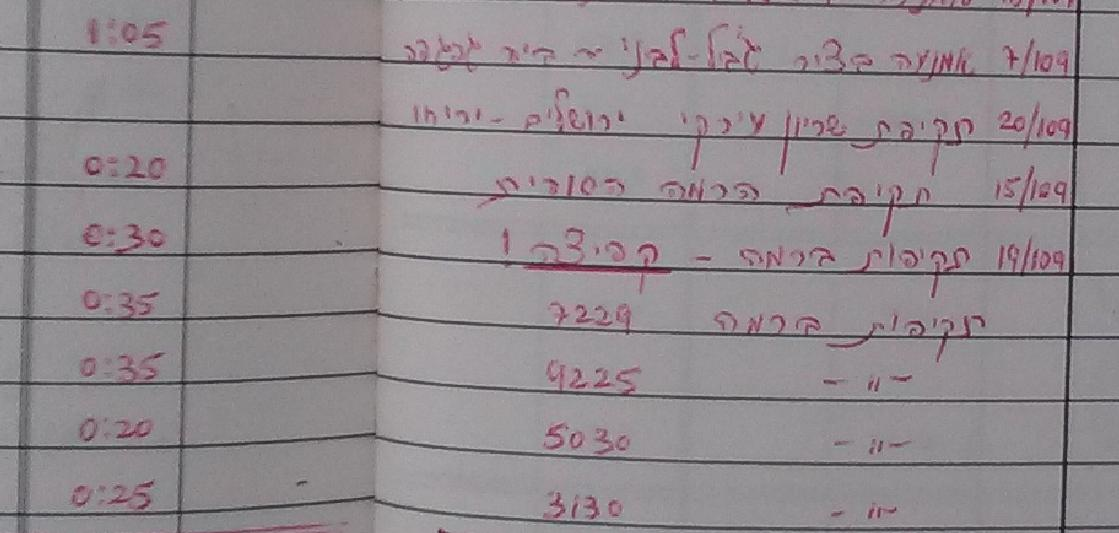
\includegraphics[scale=0.6]{History_BenNun/YhSu4RMbuBo.jpg}
	%	\label{fig:scipion} % Unique label used for referencing the figure in-text\end{document}
	%	%\addcontentsline{toc}{figure}{Figure \ref{fig:placeholder}} % Uncomment to add the figure to the table of contents%----------------------------------------------------------------------------------------
	\caption{Описание отказа самолета из лётной книжки Асафа Бен-Нуна }%	CHAPTER 2
\end{figure}

Из документов 3-й бригады на границе с Сирией: «Около 07 ч. 18 м. Израильский «Мистер» был поражен в районе киббуца, и пилот попытался вернуться (с территории Сирии — А.Н.), но был вынужден покинуть самолет прямо на границе. Это был драматический момент, когда сирийцы стреляли в катапультировавшегося пилота, в то время как наши силы пытались спасти его. … Чтобы спасти пилота, который приземлился в нескольких метрах к западу от Иордана, командир 32 батальона отправился туда, чтобы вытащить его из-под носа сирийцев.

Заместителем командира подразделения был майор Узи Котлер, но первым, кто прибыл в Бен-Нуну, был капитан Шай Арази, командир роты в 32 батальоне. Он легко вспоминает детали инцидента и с большой точностью описывает его. «Это было в районе кибуца Гадот, который считался критически важной областью с точки зрения намерений Сирии атаковать Израиль оттуда. Мы обороняли три форпоста под дорогой, ведущей к мосту Бнот Яаков, в районе ДМЗ, вместе с подразделением пограничной полиции».

Арази рассказывает: «Мы внезапно увидели «Мистер» с черным дымом, который медленно летел на запад, а затем упал возле кибуца. Затем мы увидели пилота на парашюте. Мы все встали и смотрели, на какую сторону Иордана от упадет, потому что за мостом сидели сирийцы. Ночью я лежал в засаде в десяти метрах от моста»

«В какой-то момент я понял, что пилот падает на нашу сторону, и я сел в джип, и поехал к нему, в тот район, где была старая таможня. Я помню, как там были другие джипы, и я был с моим водителем, Ициком, парнем из Рош-Пины, только мы вдвоем, без связи или чего-то еще, мы поехали вниз, мы добрались туда, а затем мы увидели пилота. Я думал, его ранили, потому что он не мог встать на ноги, так что я схватил его за штаны и втащил в джип, так что его ноги свисали с джипа, и я сказал водителю побыстрее убираться отсюда. Я вернул лётчика и вернулся к своим обязанностям. Я не придавал слишком большого значения событию».

Бен-Нун рассказывает: «Там были развалины старой таможни, где находился джип пограничной полиции, оно отвел меня в полицейский участок Рош-Пина, где меня осмотрел доктор. Эта поездка была самой опасной частью всего этого, потому что водитель, кажется, решил, что тоже умеет летать. Но по обеим сторонам дороги стояли сотни или тысячи людей, это были силы, которые собирались атаковать Голанские высоты. Солнце было на западе, и они все это видели. Они видели мой сбитый самолёт, как я спускался вниз, они услышали стрельбу, а затем я услышал, как многие обсуждали это. И джип летал между ними по узкой дороге, это было даже немного страшно». 

\textit{Что произошло после в Рош-Пине? }

«Оттуда они отвели меня в штаб бригады, где я встретил подполковника Мано Шейка Я знал его с тех лет. Он обнял меняи он дал мне виски. Я обычно не пью, но тот случай был особенным. Оттуда они отвезли меня на вертолете в Рамат Давид, и на следующий день я снова летал».

\begin{figure}[h!tb] 
	\centering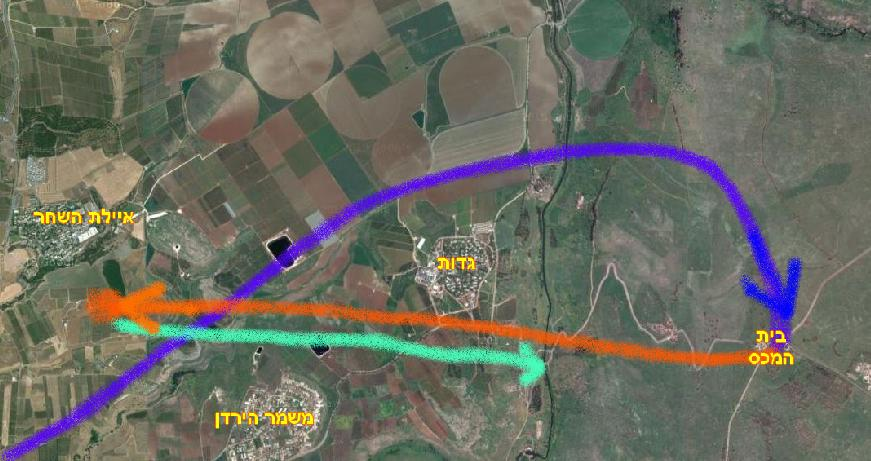
\includegraphics[scale=0.6]{History_BenNun/1O9jR38jRwA.jpg}
	%	\label{fig:scipion} % Unique label used for referencing the figure in-text\end{document}
	%	%\addcontentsline{toc}{figure}{Figure \ref{fig:placeholder}} % Uncomment to add the figure to the table of contents%----------------------------------------------------------------------------------------
	\caption{Карта вылета Асафа Бен-Нун 7 июня 1967 года. 1) Маршрут атаки цели (синий). 2) Самолет был сбит около старой таможни, и Бен-Нун направил его на территорию Израиля (красный). 3) Ветер относит парашют Бен-Нуна после катапультирования (зелёный). }%	CHAPTER 2
\end{figure}

Бен-Нун вернулся ночью к авиабазе Рамат-Дэвида, получил день отдыха, а в пятницу, 9 июня, когда началось большое сражение на сирийском фронте, он организовал себе один вылет, чтобы атаковать цель 7229 [артиллерийское соединение вблизи перекрестка Нафах]. Он завершил войну в сирийском секторе 10 июня с тремя вылетами, чтобы атаковать цели 9225 [позиция артиллерийской батареи в 700 метрах к югу от Сахады], 5030 [форпост перед Альмагором] и 3130 [артиллерийский состав к югу от Верхнего Тауфика].

О нападениях 9 июня на сирийскую территорию он рассказывает: «Мы атаковали волнами, и диспетчер заставил нас ждать на высотах над Сафедом, потому что в этот день «Фуги» (Фуга Маджистер, учебно-боевой самолёт лётной школы - А.Н.) выполняли своё задание, все мы были на одном канале. Я хорошо знал того парня, его звали Арье Бар-Ор (Орбах), он объявляет «захожу на цель», а потом его номер два говорит — «первый номер столкнулся в землёй». Арье, командир эскадрильи «Фуг» погиб, и их полёты прекратили.

\textit{Когда вы получили еще одну задачу для атаки в сирийском секторе, в районе недалеко от таможни, вы не волновались?}

«Ничего, нет, это война»

\textit{Что вы видели, что случилось с «Мистером» после того, как вы его покинули?}

Он упал на холм к югу от Айеле Хашахара. После войны они пригласили меня в киббуц, чтобы рассказать эту историю и привезли части самолета. Через несколько дней после войны мне позвонил мой хороший друг, который был на Киббуце Гадот, и он сказал мне: «Послушай, я знаю, где он — приходи и забирай его». У меня был Fiat 600 с тентом, я пришел, я положил кресло на крышу, а там недалеко был контрольно-пропускной пункт военной полиции, который досматривал солдат, возвращающихся из Сирии. Меня арестовали, и я рассказал им эту историю. Мне потребовалось много времени, чтобы убедить их, что это от моего самолёта. На протяжении многих лет кресло был в моем доме, и дети сидели на нем и играли с ним».

Другая история, которую он помнит: через день или два после войны «Пайпер» (лёгкий самолёт ВВС — А.Н.) приземлился в Рамат-Давиде, а оттуда прибыли два генерала запаса — мой брат Йохай Бен-Нун и Меир Зореа. Асаф Бен-Нун рассказывает : «Меир Зореа попросил сопровождать их, чтобы найти сына Йона (Йонатан Зореа, также пилот «Мистера» разбился 5 июня 1967 года, пытаясь вернуться на повреждённом «Мистере» из Сирии — А.Н.), пилота, который упал на Голанских высотх, но командир эскадрильи не отпустил меня».

\begin{figure}[h!tb] 
	\centering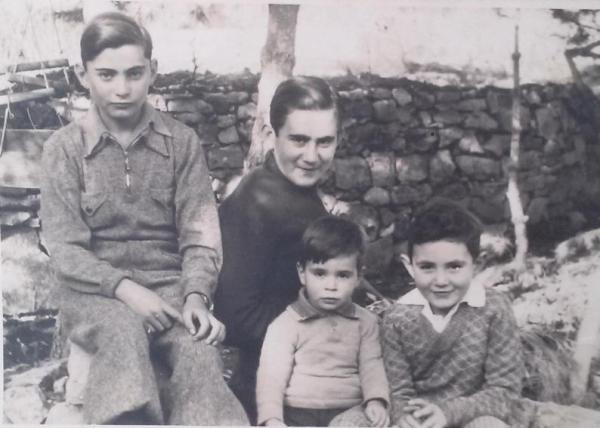
\includegraphics[scale=0.6]{History_BenNun/OfI9-eAh-Ag.jpg}
	%	\label{fig:scipion} % Unique label used for referencing the figure in-text\end{document}
	%	%\addcontentsline{toc}{figure}{Figure \ref{fig:placeholder}} % Uncomment to add the figure to the table of contents%----------------------------------------------------------------------------------------
	\caption{Братья Бен-Нун в их доме в Бейт-Хакереме 1940 года. Справа: Нери, Ассаф, Шмуэль и Йохай. }%	CHAPTER 2
\end{figure}

«Я помню эйфорию, которая преобладала после войны, особенно в ВВС, когда они носили летчиков на руках, но я был совершенно трезв, даже тогда я сказал, что не стоит почивать на лаврах. Скажем так: Война Судного дня - это война Судного дня, это великая травма. Я был на «Рааме» - Мираже, сделанном в Израиле, и три дня я не покидал кабину, почти не ел и не пил. Это была война не на жизнь, а насмерть. Когда вы в бою, вы как рыцари - или вы, или он.

Шестидневная война начались и сразу закончилсь, она была интенсивной, но я не испытывал таких переживаний. Мои два брата, Йохаи и Нери, были в круизе в районе Крита или Родоса, как спортсмены, и мы искали их в течение трех дней, не имели контакта с ними из-за шторма, и я очень волновался».

\textit{Были ли у вас кошмары?}

«У меня не было кошмаров».

В течение 30 лет он был пилотом IAI в проектах «Лави» и «Кфир». Он служил в течение 4,5 лет в качестве командира Boeing 727 миллиардера Шауля Эйзенберга («Удивительные годы, мы летали по всему миру»), за три года до его ухода на пенсию.

\begin{figure}[h!tb] 
	\centering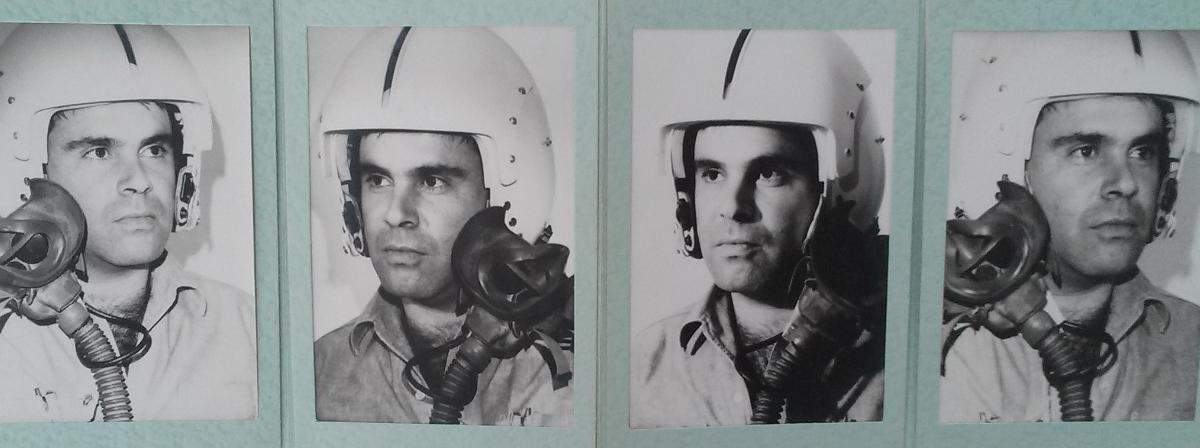
\includegraphics[scale=0.4]{History_BenNun/5o7jnb-c_8Y.jpg}
	%	\label{fig:scipion} % Unique label used for referencing the figure in-text\end{document}
	%	%\addcontentsline{toc}{figure}{Figure \ref{fig:placeholder}} % Uncomment to add the figure to the table of contents%----------------------------------------------------------------------------------------
	\caption{Пилот собрал Бен-Нун в 1967 году.  }%	CHAPTER 2
\end{figure}


\textit{ Со всем своим опытом, как военный и гражданский пилот с тысячами летных часов на многих типах самолетов, какой совет вы могли бы дать молодому пилоту Асафу Бин-Нуну, когда он был сбит над сирийской границей?}

Я делал то, что должен был сделать, а не что-то необычное ... Послушай, я могу быть уверенным, что в таких ситуациях я и тогда был хладнокровен.

И что он делал с тех пор, как ушел на пенсию? «Прошло 15 лет с тех пор, как я начал наслаждаться этим, и в возрасте 70 лет я научился играть на саксофоне, и это необыкновенное удовольствие. Я не скучаю по полётам. Это хорошо для меня, мне нравится жизнь».

На этом интервью заканчивается. 

Во время Войны Судного дня Бин-Нун сбил четыре самолёта, три МиГ-21 и один Су-7 в качестве пилота-резервиста эскадрильи «Миражей».

\begin{figure}[h!tb] 
	\centering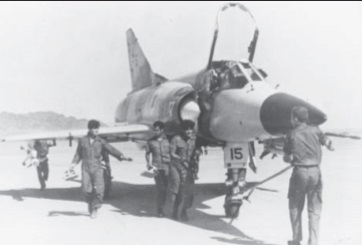
\includegraphics[scale=0.8]{History_BenNun/ypM9yR7fsDQ.jpg}
	%	\label{fig:scipion} % Unique label used for referencing the figure in-text\end{document}
	%	%\addcontentsline{toc}{figure}{Figure \ref{fig:placeholder}} % Uncomment to add the figure to the table of contents%----------------------------------------------------------------------------------------
	\caption{«Нешер» №15, на котором была одержана вторая победа, 6 октября 1973. }%	CHAPTER 2
\end{figure}

Свою первую победу он описывает так:

«Мы увидели четверку Су-7 на малой высоте, Эрми (ведущий пары) был чуть-чуть впереди меня, и сильно справа. Я был позади Су-7, в отличном положении, так что я выпустил ракету сразу, как только услышал жужжание, говорившее о том, что ГСН захватила цель. Я нажал на кнопку пуска — но ничего не случилось. Су-7 летел низко, и поднимал много пыли и песка. В нажал на переключатель другой ракеты. Было странно — я не видел цели, но всё ещё слышал жужжание. Эрми был справа — значит, я точно не мог поразить его, так что я всё-же выпустил ту ракету, проследил за ней, и увидел большой взрыв».

После Войны Судного дня, Асаф Бен-Нун продолжил работу в качестве лётчика-испытателя концерна IAI. Его основной «зоной ответственности» был проект «Кфир» — создание нового израильского лёгкого истребителя-бомбардировщика на базе «Миража». 

\begin{figure}[h!tb] 
	\centering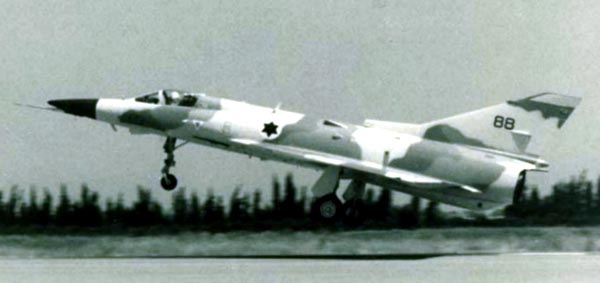
\includegraphics[scale=0.8]{History_BenNun/jceZ2lxQ9no.jpg}
	%	\label{fig:scipion} % Unique label used for referencing the figure in-text\end{document}
	%	%\addcontentsline{toc}{figure}{Figure \ref{fig:placeholder}} % Uncomment to add the figure to the table of contents%----------------------------------------------------------------------------------------
	\caption{Нэшер номер 88 с личным именем "Раам" (гром). }
	%	\caption{Нэшер номер 88 с личным именем "Раам" (гром). Один из первых прототипов "Кфира"}%	CHAPTER 2
\end{figure}

25 мая 1975 года, в ходе тестового полёта, прототип нового самолёта потерпел крушение над Средиземным морем. Бен-Нуну удалось спастись, это было его второе катапультирование из повреждённого самолёта.

\begin{figure}[h!tb] 
	\centering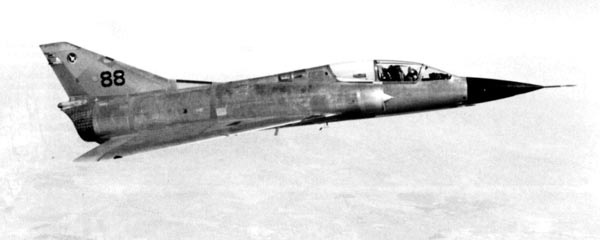
\includegraphics[scale=1.0]{History_BenNun/9TjHoDK-tYw.jpg}
	%	\label{fig:scipion} % Unique label used for referencing the figure in-text\end{document}
	%	%\addcontentsline{toc}{figure}{Figure \ref{fig:placeholder}} % Uncomment to add the figure to the table of contents%----------------------------------------------------------------------------------------
	\caption{"Технолог", самолёт на базе "Миража", использовался для тестирования вносимых в аэродинамику изменений }%	CHAPTER 2
\end{figure}

В 1974-м он был членом израильской делегации в США, занимавшейся выбором нового самолёта для ВВС Израиля. Асаф провел пару полётов на TF-15 \#71-0290. В обоих его сопровождали американские коллеги — в задней кабине «Орла».

Ассаф так это вспоминал: «Я был сотрудником IAI и лётчиком-резервистом ВВС, когда стал членом команды по выбору нового самолёта в качестве лётчика-испытателя, по прямому указанию главкома ВВС Бени Пеледа. Сначала мы «летали» на симуляторах - симуляторе кабине и симуляторе боя. Оба были чертовски реалистичными.

Во время первого настоящего полёта, я попытался захватить цель радаром за пределами визуального обнаружения, и "использовал" пару ракет с полуактивным радарным наведением. Потом, ближе — пару ракет с инфракрасной ГСН и пушку. Обе атаки были успешными — в одном единственном заходе на моего оппонента. Это был самолёт-откровение, с потрясающей маневренностью и скоростью. Единственным моим замечанием были его размеры - я предпочитал истребители поменьше». К слову, «оппонентом» был «Фантом», который пилотировал другой израильтянин — Омри Офек.

Потом израильтяне переместились в Мирамар, где находилась знаменитая флотская школа «Топ Ган», и провёл несколько учебных боёв с другим претендентом — F-14. Теперь — уже в качестве «оппонента», пилотируя двухместный «Скайхок». С «Котом» вышло сложнее — в ближнем бою «Скайхок» вышел победителем. Потом Бин-Нун оказался уже в кабине «Кота» - с флотским пилотом Кейтом Шиханом (Keith Sheehan) на «заднем сидении»:

«F-14 не хватало тяговооруженности, он был сложный, он был недружелюбный (имеется в виду, более сложный в пилотировании — А.Н.), и он не был аэродинамически чист. Кроме того, он дрожал на больших углах атаки и перегрузках. Во время моего вылета, моим противником был Амнон Арад на «Скайхоке», и мы закончили с равным счётом. В это трудно поверить, но в ближнем бою F-14 уступал «Скайхоку»...

В итоге, оптимизированный для перехвата целей на большом расстоянии F-14 проиграл F-15. Единственное преимущество «Кота», возможность поразить противника с огромного расстояния, была просто излишней для Израиля, в остальном — же F-15 был лучше, или как минимум не хуже. А ещё «Орёл» был существенно дешевле — и при покупке, и в обслуживании.

Через пять лет после учебных воздушных боёв в Сент-Луисе, Мирамаре и Сан-Диего, израильские F-15 вступили в настоящие — с сирийскими МиГ-21 над Ливаном. Исход был предрешен, опытнейшие пилоты «Миражей», получившие новые самолёты, не оставили сирийцам шансов. Тогда-же, в сентября 79-го, первую (и единственную) победу одержал «Кфир». Так получилось, что к появлению обоих этих самолётов в Израиле приложил руку Ассаф Бин-Нун...

\begin{figure}[h!tb] 
	\centering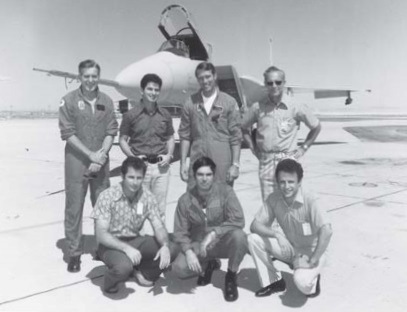
\includegraphics[scale=0.8]{History_BenNun/eccw4mb3YRI.jpg}
	%	\label{fig:scipion} % Unique label used for referencing the figure in-text\end{document}
	%	%\addcontentsline{toc}{figure}{Figure \ref{fig:placeholder}} % Uncomment to add the figure to the table of contents%----------------------------------------------------------------------------------------
	\caption{Асаф Бин-Нун (второй, сидит) в США с лётчиками фирмы Макдонелл-Дуглас, и прототипом F-15, 1974 год}%	CHAPTER 2
\end{figure}

Источники: \cite{bennun_inter,segev,misnikov,kuper_nikole}

Ссылка на оригинал \url{https://vk.com/wall-162479647_38820}

К оглавлению на странице \pageref{tablecont}